\documentclass{article}
\usepackage[utf8]{inputenc} %кодировка
\usepackage[T2A]{fontenc}
\usepackage[english,russian]{babel} %русификатор 
\usepackage{mathtools} %библиотека матеши
\usepackage[left=1cm,right=1cm,top=2cm,bottom=2cm,bindingoffset=0cm]{geometry} %изменение отступов на листе
\usepackage{amsmath}
\usepackage{graphicx} %библиотека для графики и картинок
\graphicspath{}
\DeclareGraphicsExtensions{.pdf,.png,.jpg}
\usepackage{subcaption}
\usepackage{pgfplots}
\usepackage{float}

\begin{document}
% НАЧАЛО ТИТУЛЬНОГО ЛИСТА
\begin{center}
    \Large
    Федеральное государственное автономное \\
    образовательное учреждение высшего образования \\ 
    «Научно-образовательная корпорация ИТМО»\\
    \vspace{0.5cm}
    \large
    Факультет программной инженерии и компьютерной техники \\
    Направление подготовки 09.03.04 Программная инженерия \\
    \vspace{1cm}
    \Large
    \textbf{Отчёт по лабораторной работе №3} \\
        По дисциплине «Компьютерные сети» ( семестр 6)\\
    \large
    \vspace{8cm}

    \begin{minipage}{.33\textwidth}
    \end{minipage}
    \hfill
    \begin{minipage}{.4\textwidth}
    
        \textbf{Студент}: \vspace{.1cm} \\
        \ Дениченко Александр P3312\\
        \textbf{Практик}:  \\
        \ Тропченко Андрей Александрович
    \end{minipage}
    \vfill
Санкт-Петербург\\ 2025 г.
\end{center}
\pagestyle{empty}
% КОНЕЦ ТИТУЛЬНОГО ЛИСТА 
\newpage
\pagestyle{plain}

\section*{Цель работы}
Изучение принципов конфигурирования и процессов функционирования
компьютерных сетей, представляющих собой несколько подсетей, связанных с
помощью маршрутизаторов, процессов автоматического распределения сетевых
адресов, принципов статической маршрутизации и динамической маршрутизации, а также передачи данных на основе протоколов UDP и TCP.

\section*{Сеть с одним маршрутизатором}
\begin{center}
    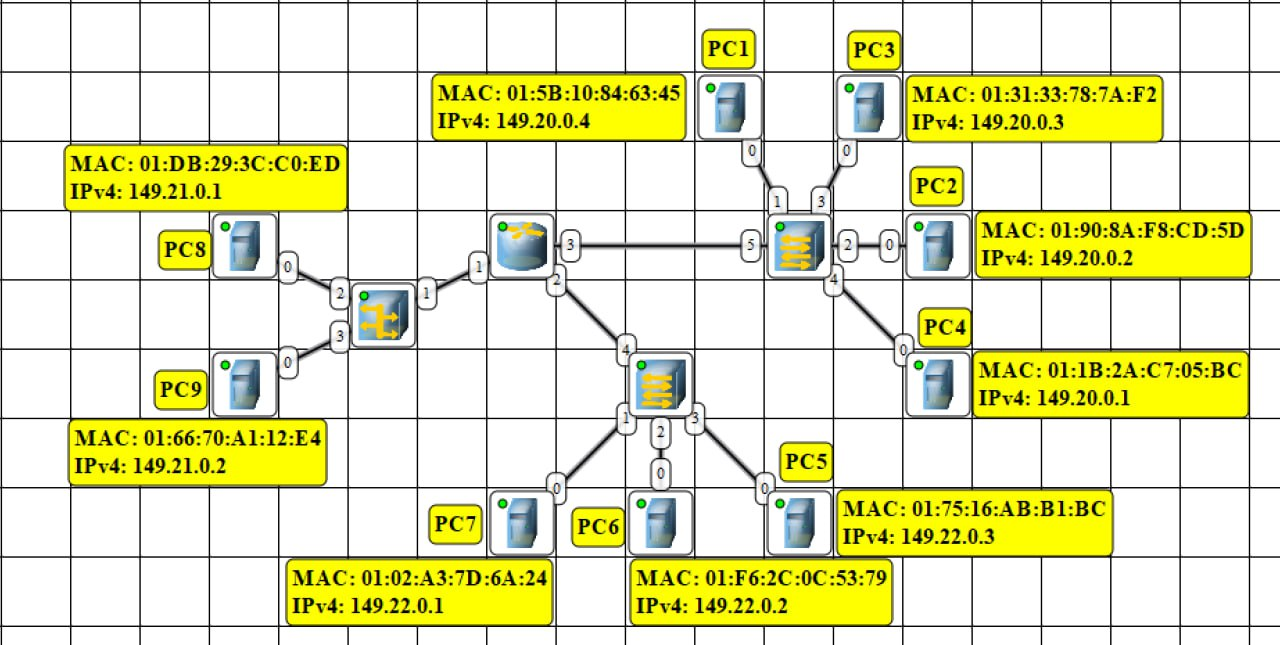
\includegraphics[width=.9\textwidth]{1-1}
\end{center}
\begin{center}
    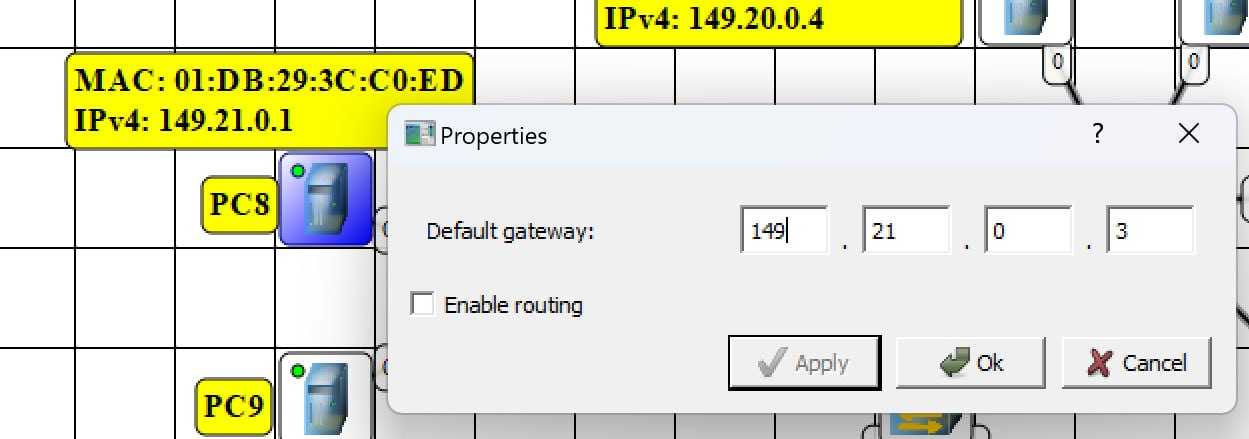
\includegraphics[width=.9\textwidth]{1-2}
\end{center}
\begin{center}
    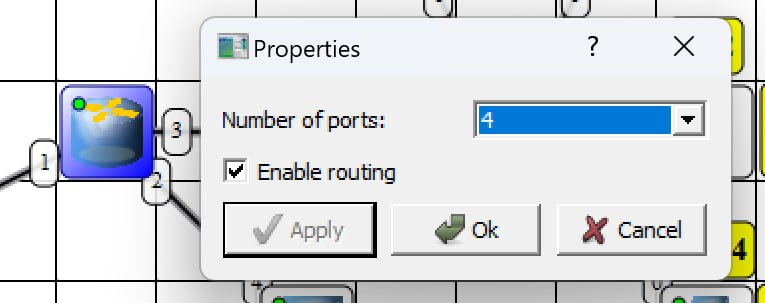
\includegraphics[width=.9\textwidth]{1-3}
\end{center}
\begin{center}
    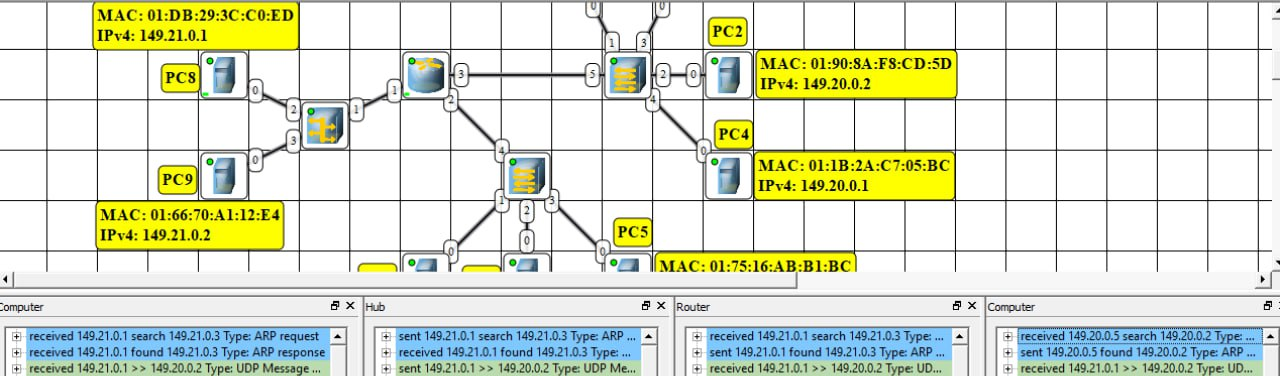
\includegraphics[width=.9\textwidth]{1-4}
\end{center}
\begin{center}
    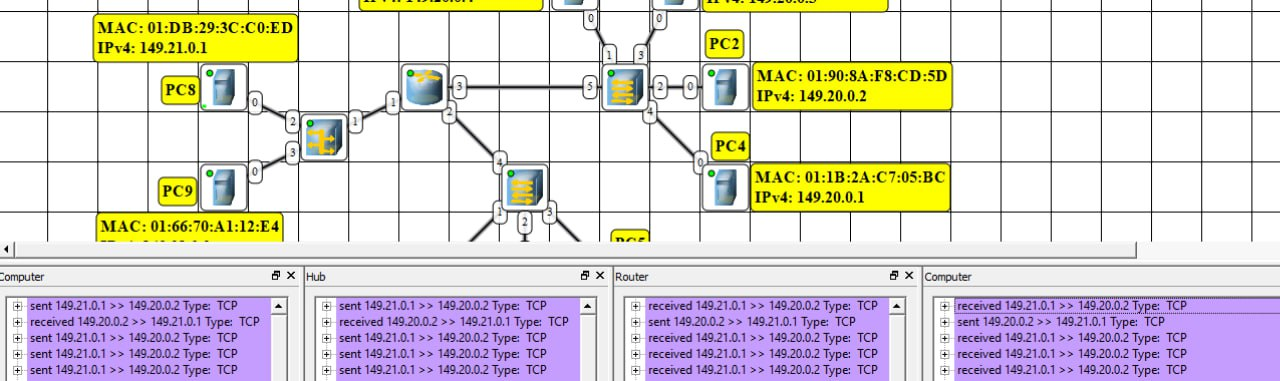
\includegraphics[width=.9\textwidth]{1-5}
\end{center}

\section*{Сеть двумя маршрутизаторами}
\begin{center}
    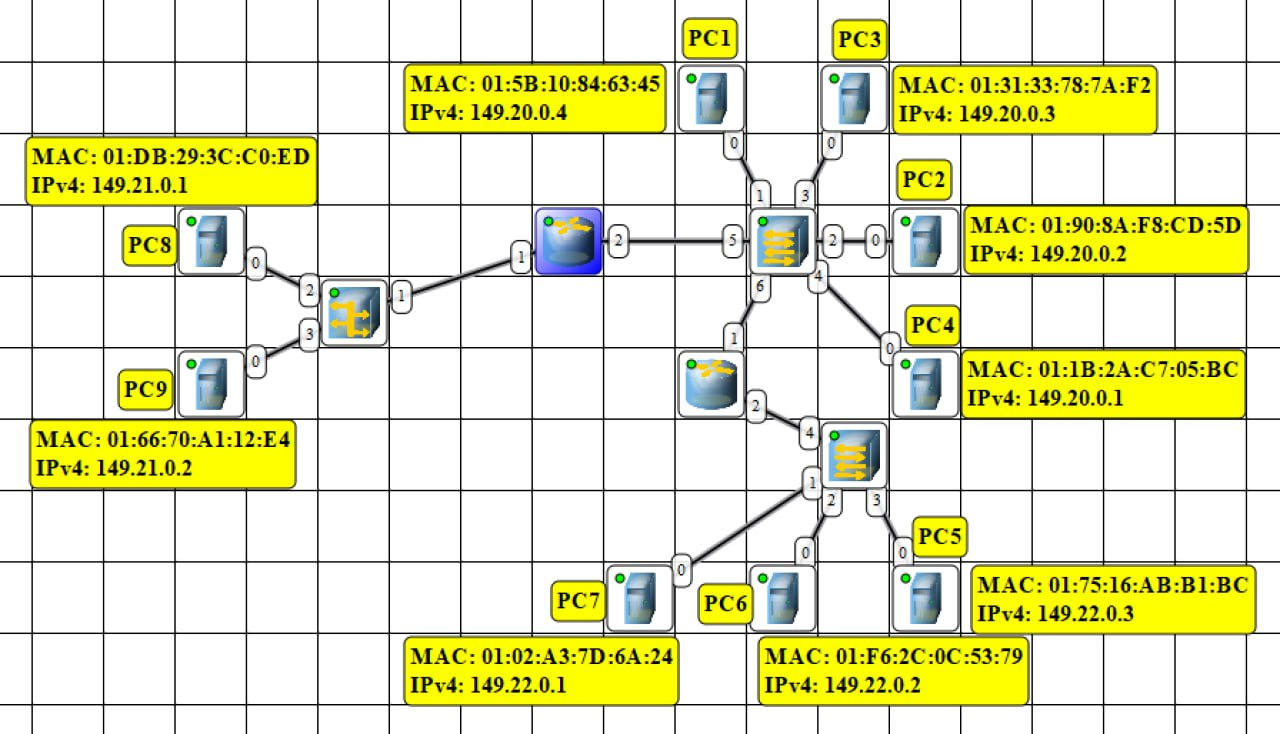
\includegraphics[width=.9\textwidth]{2-1}
\end{center}
\begin{center}
    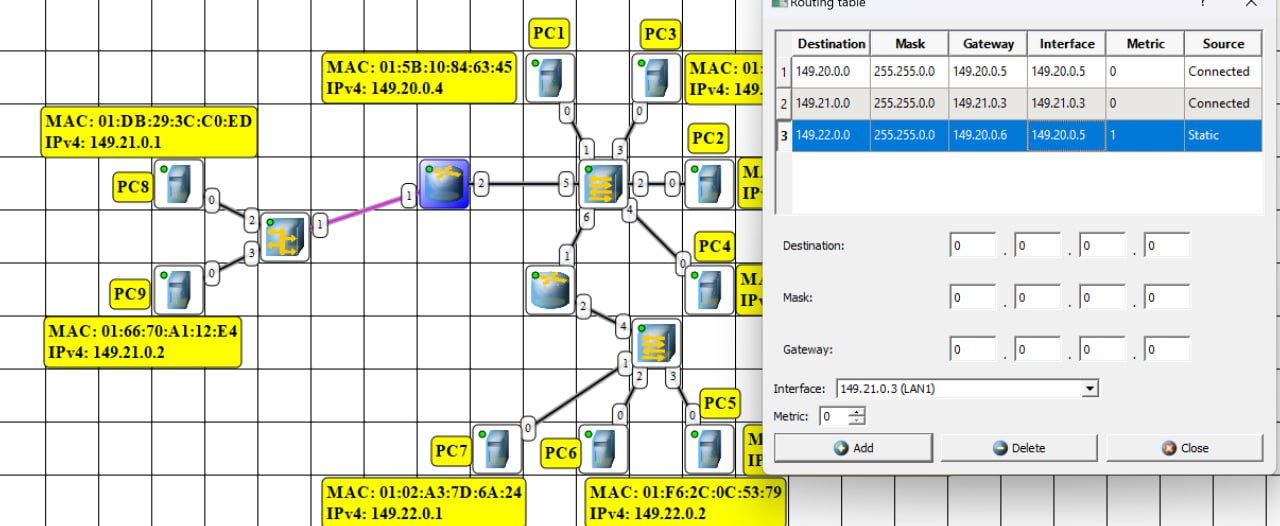
\includegraphics[width=.9\textwidth]{2-2}
\end{center}
\begin{center}
    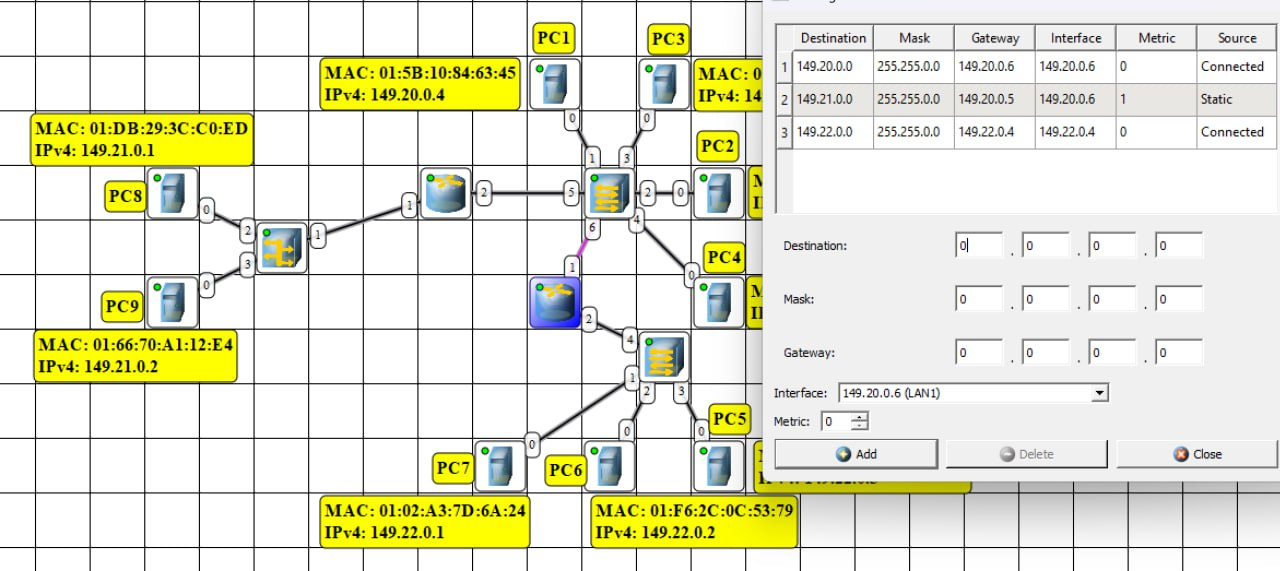
\includegraphics[width=.9\textwidth]{2-3}
\end{center}
\begin{center}
    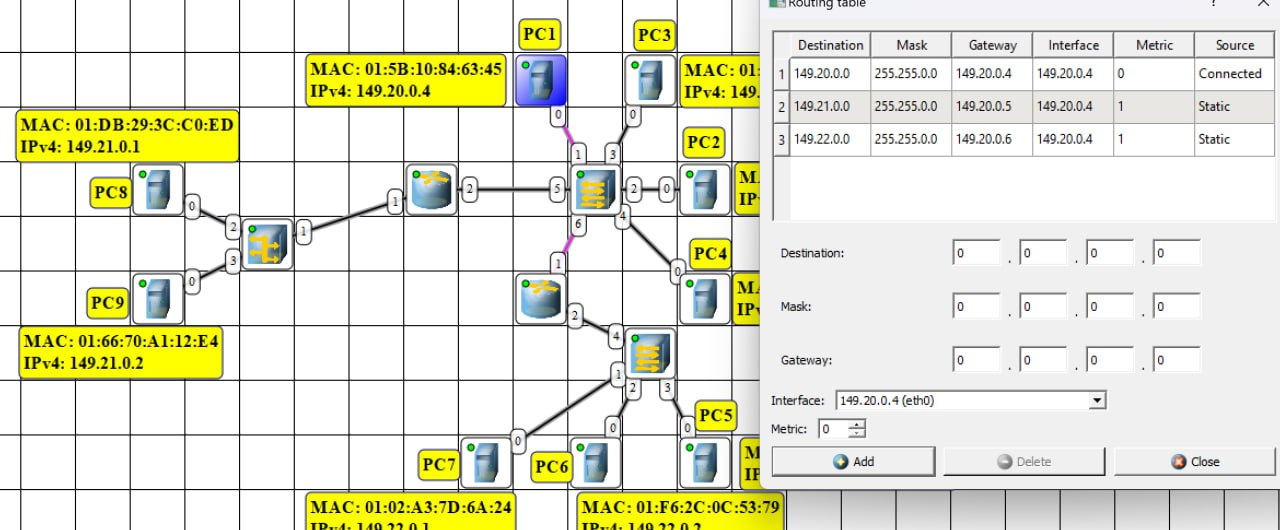
\includegraphics[width=.9\textwidth]{2-4}
\end{center}
\begin{center}
    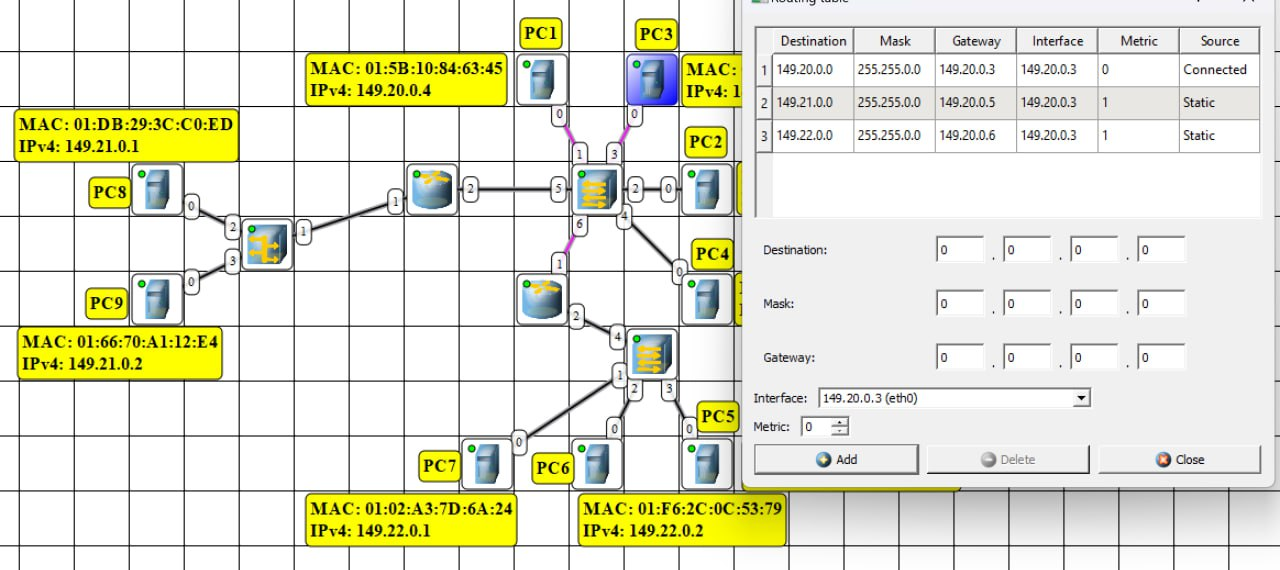
\includegraphics[width=.9\textwidth]{2-5}
\end{center}
\begin{center}
    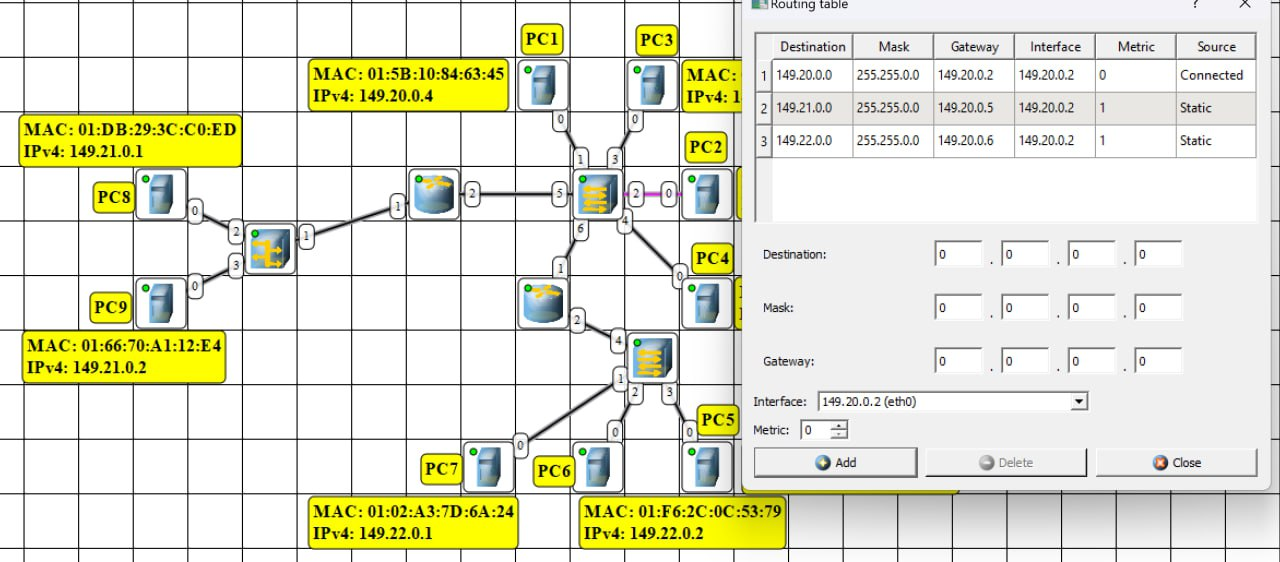
\includegraphics[width=.9\textwidth]{2-6}
\end{center}
\begin{center}
    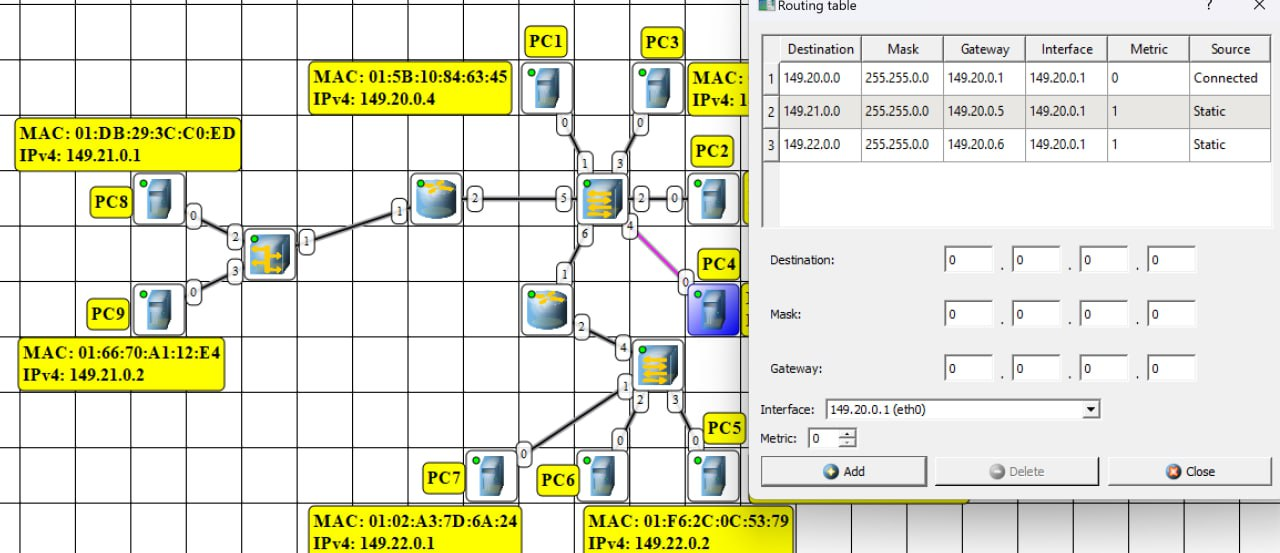
\includegraphics[width=.9\textwidth]{2-7}
\end{center}
\section*{Сеть тремя маршрутизаторами}
\begin{center}
    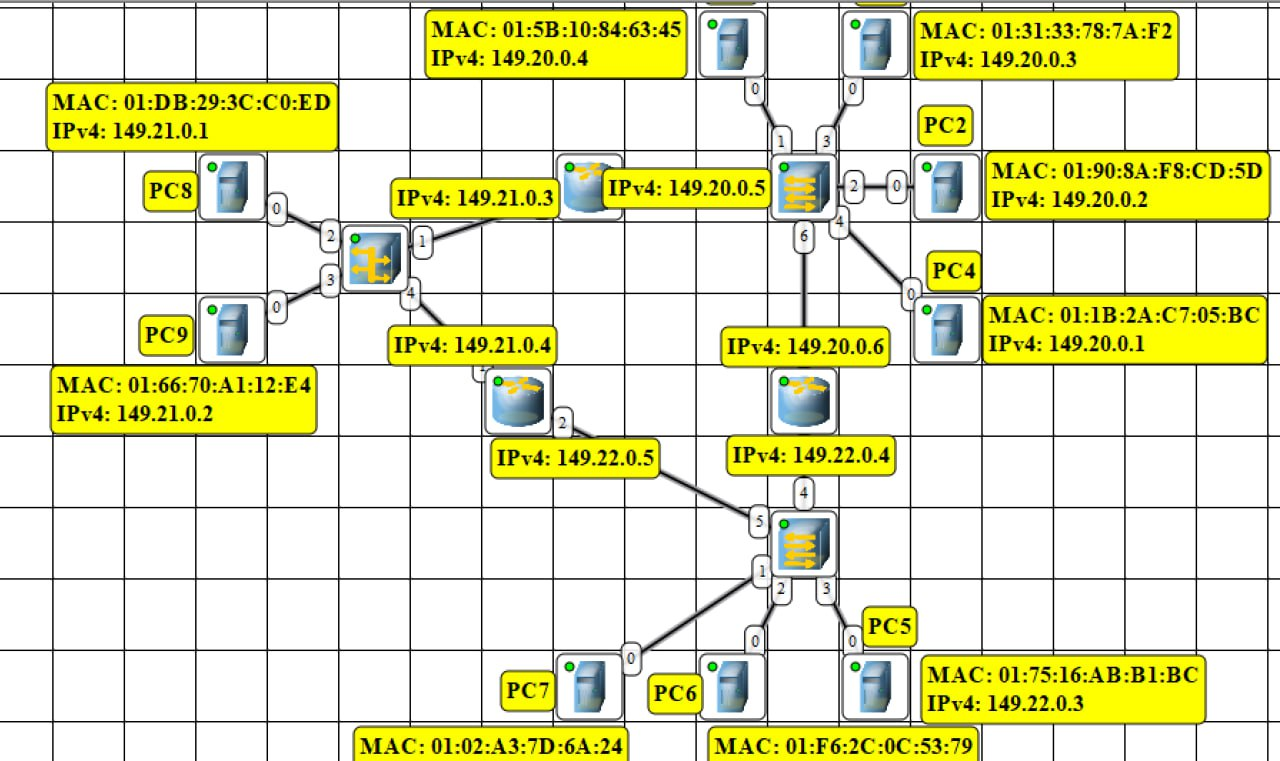
\includegraphics[width=.9\textwidth]{2-8}
\end{center}
\begin{center}
    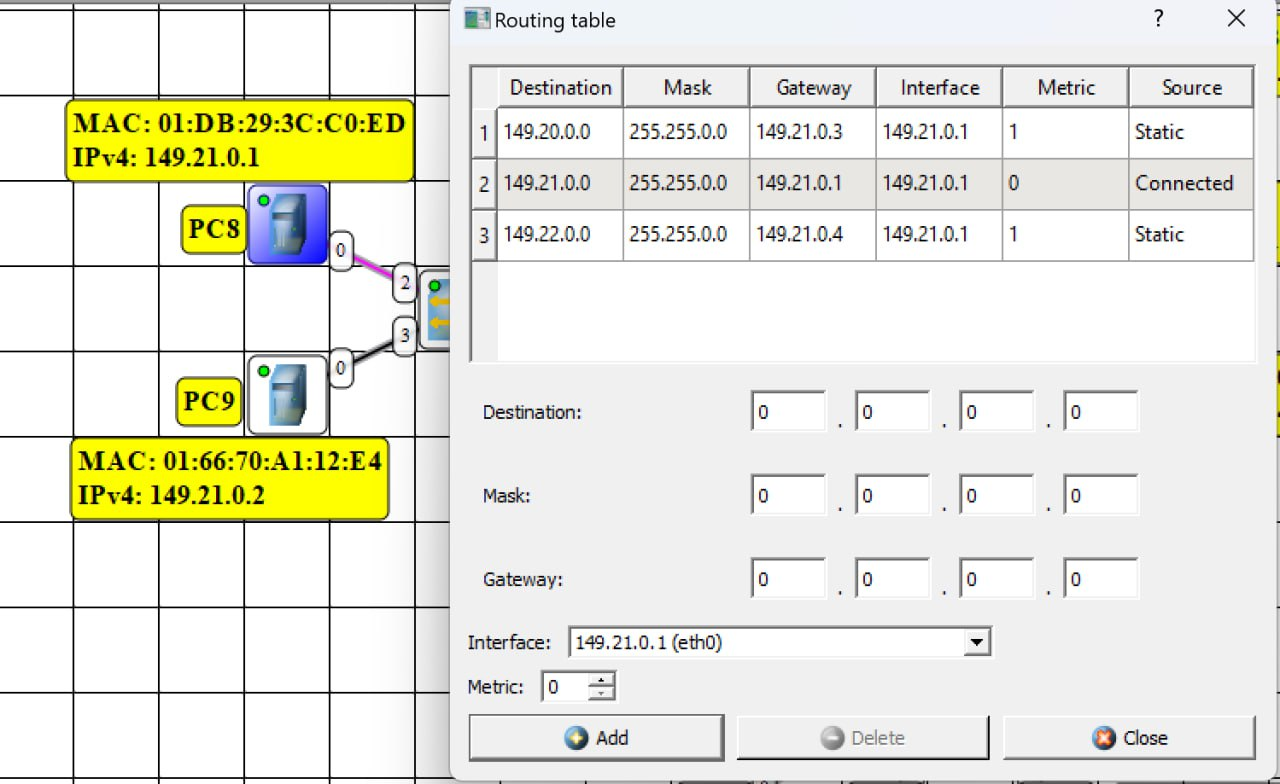
\includegraphics[width=.9\textwidth]{3-0}
\end{center}
\begin{center}
    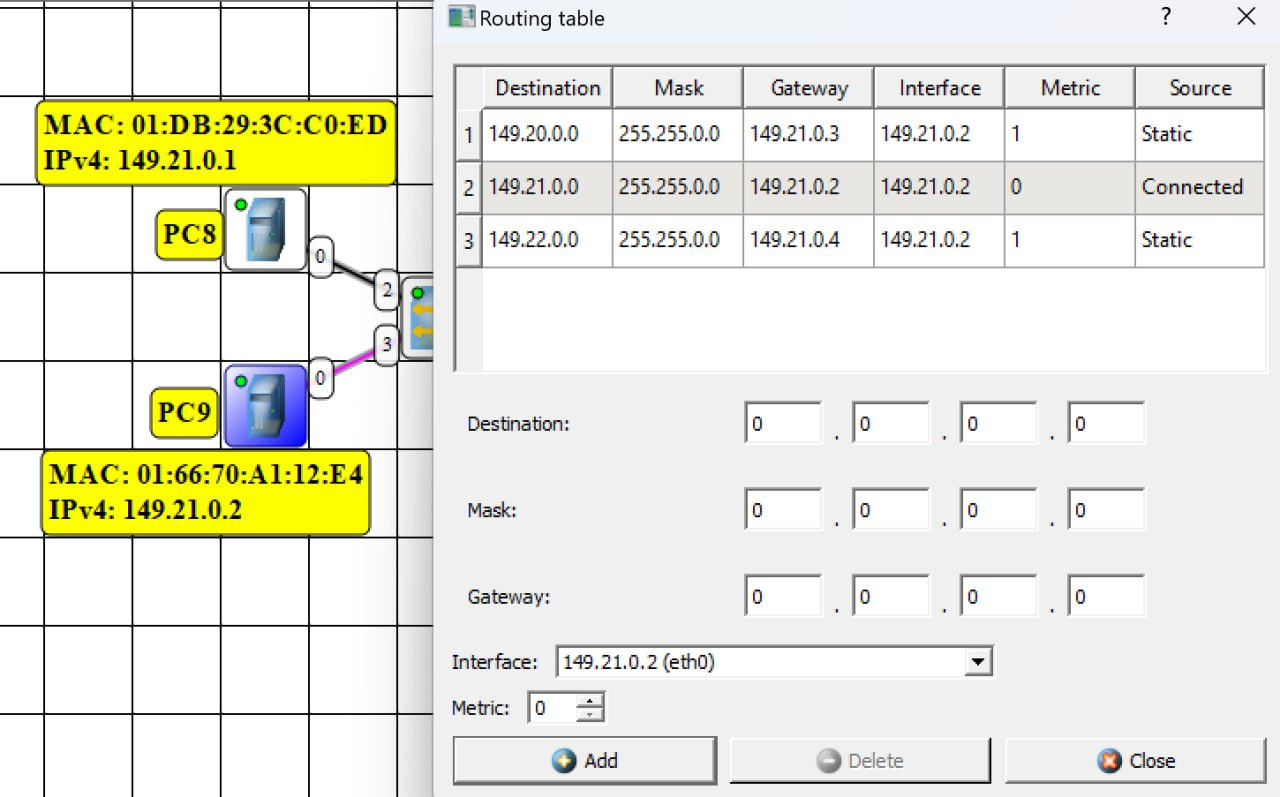
\includegraphics[width=.9\textwidth]{3-1}
\end{center}
\begin{center}
    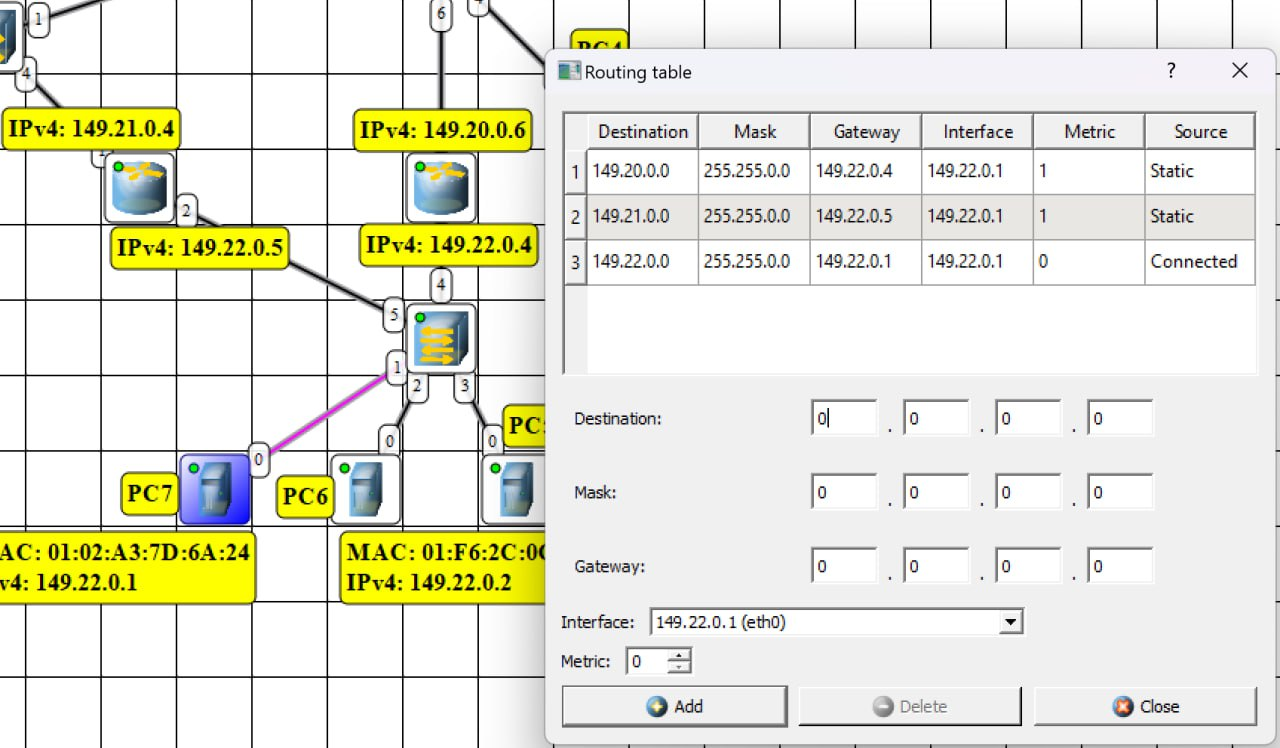
\includegraphics[width=.9\textwidth]{3-2}
\end{center}
\begin{center}
    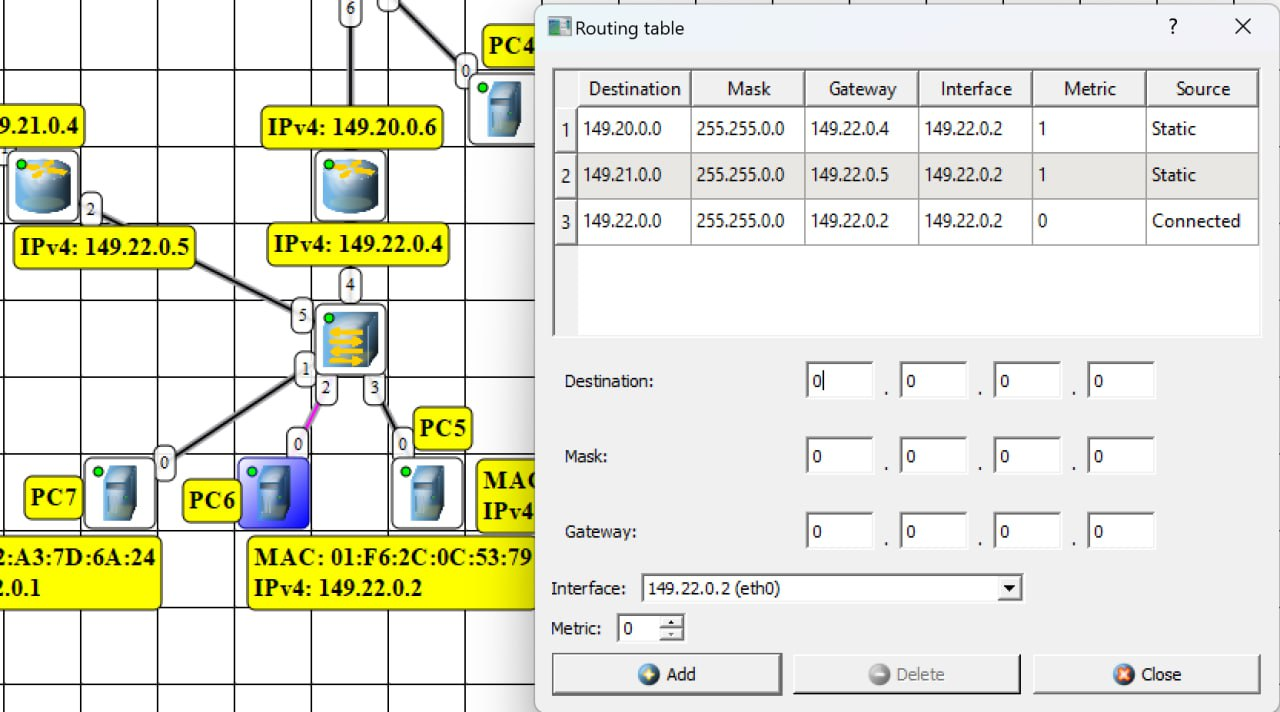
\includegraphics[width=.9\textwidth]{3-3}
\end{center}
\begin{center}
    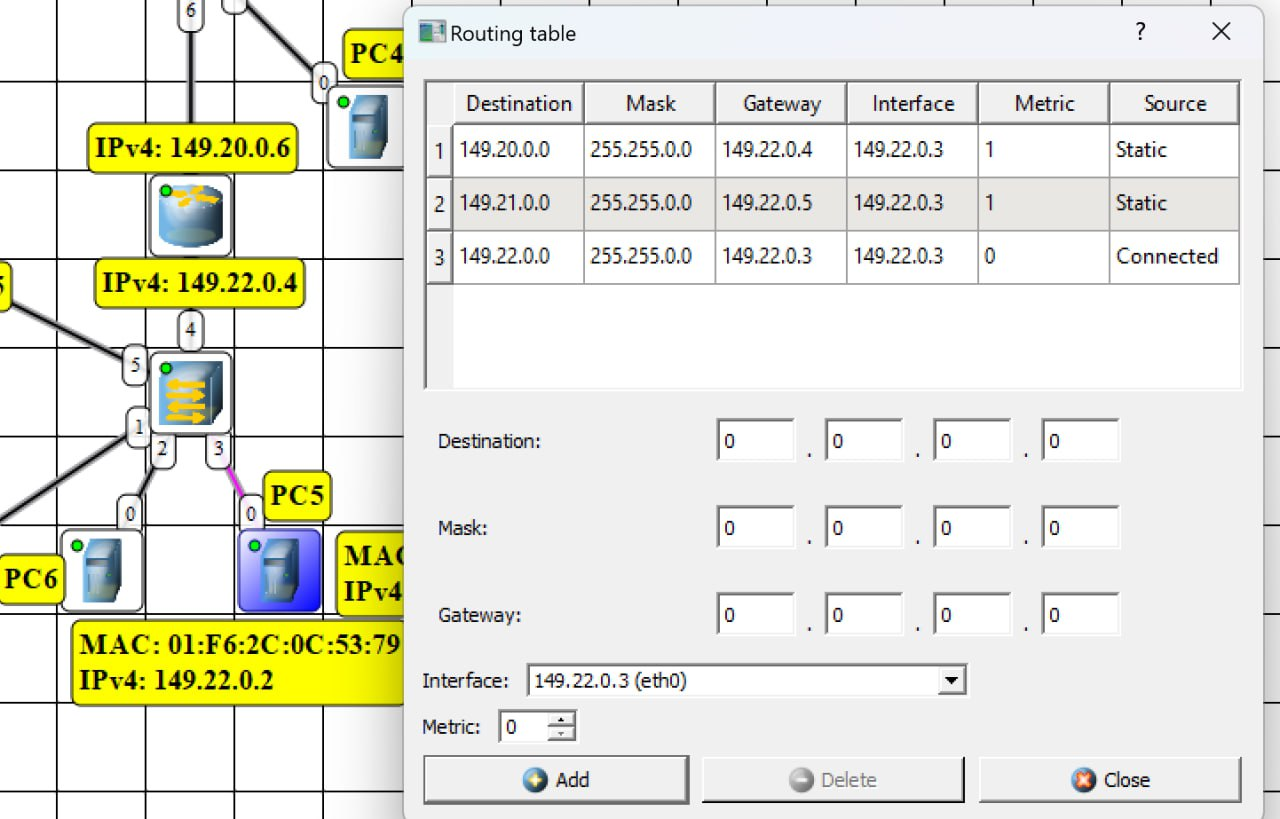
\includegraphics[width=.9\textwidth]{3-4}
\end{center}
Зацикливание
\begin{center}
    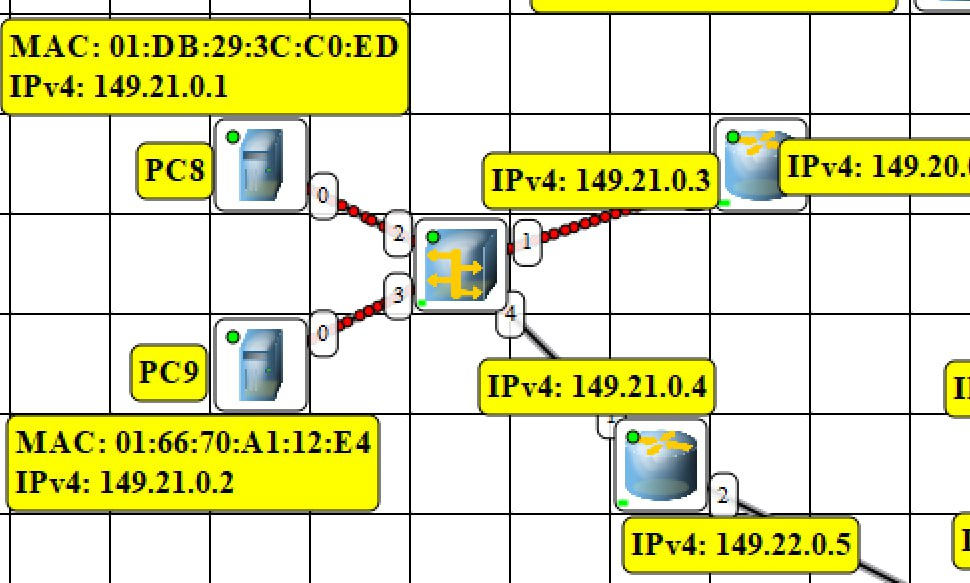
\includegraphics[width=.9\textwidth]{3-5}
\end{center}
Решение -- замена концентратора на коммутатор
\begin{center}
    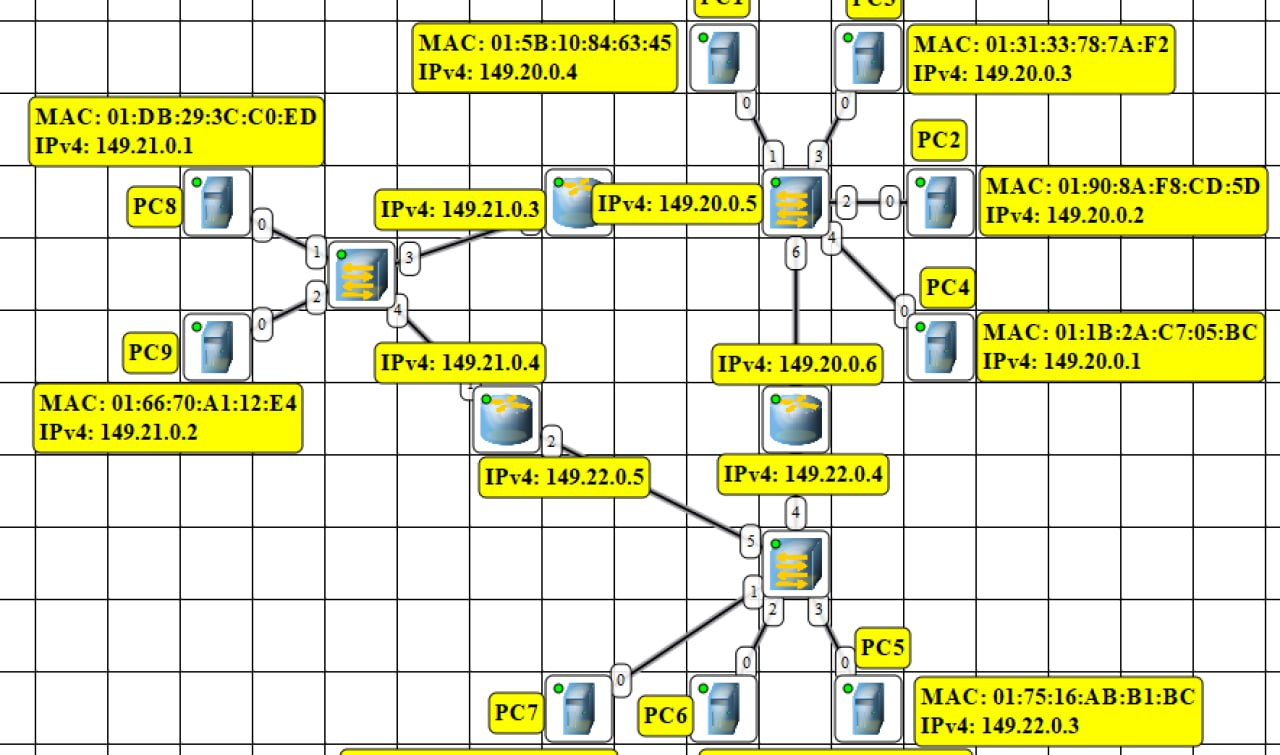
\includegraphics[width=.9\textwidth]{3-6}
\end{center}
\section*{RIP}
\begin{center}
    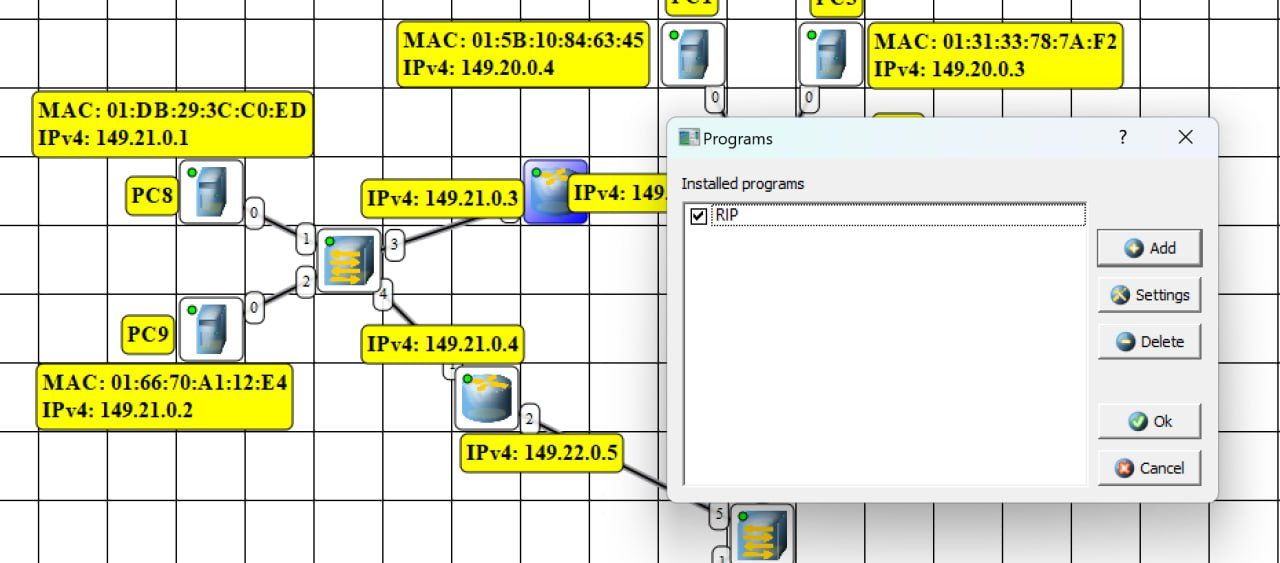
\includegraphics[width=.9\textwidth]{3-7}
\end{center}

\section*{Выход из строя одного маршрутизатора при включённом RIP}
\begin{center}
    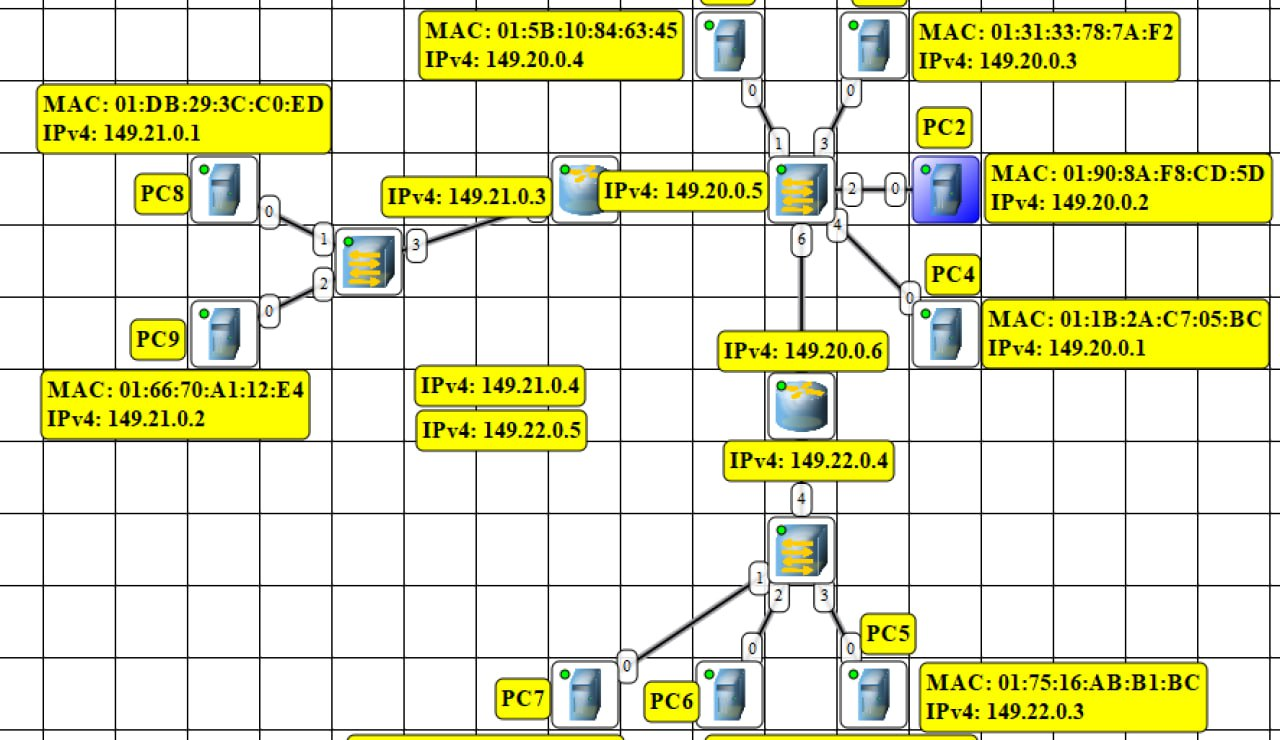
\includegraphics[width=.9\textwidth]{3-8}
\end{center}
\begin{center}
    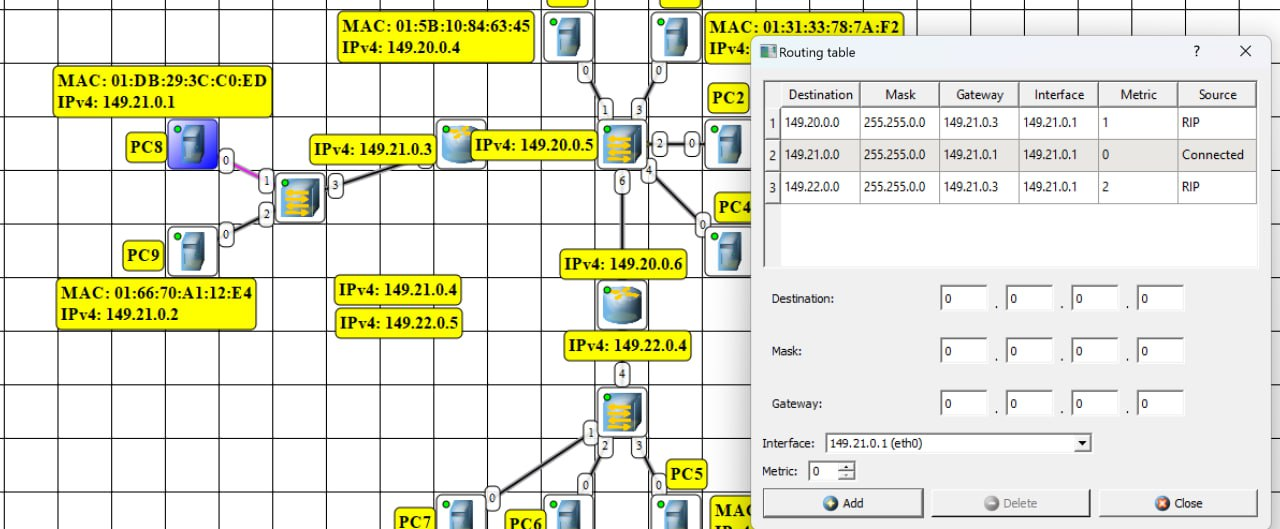
\includegraphics[width=.9\textwidth]{3-9}
\end{center}
\begin{center}
    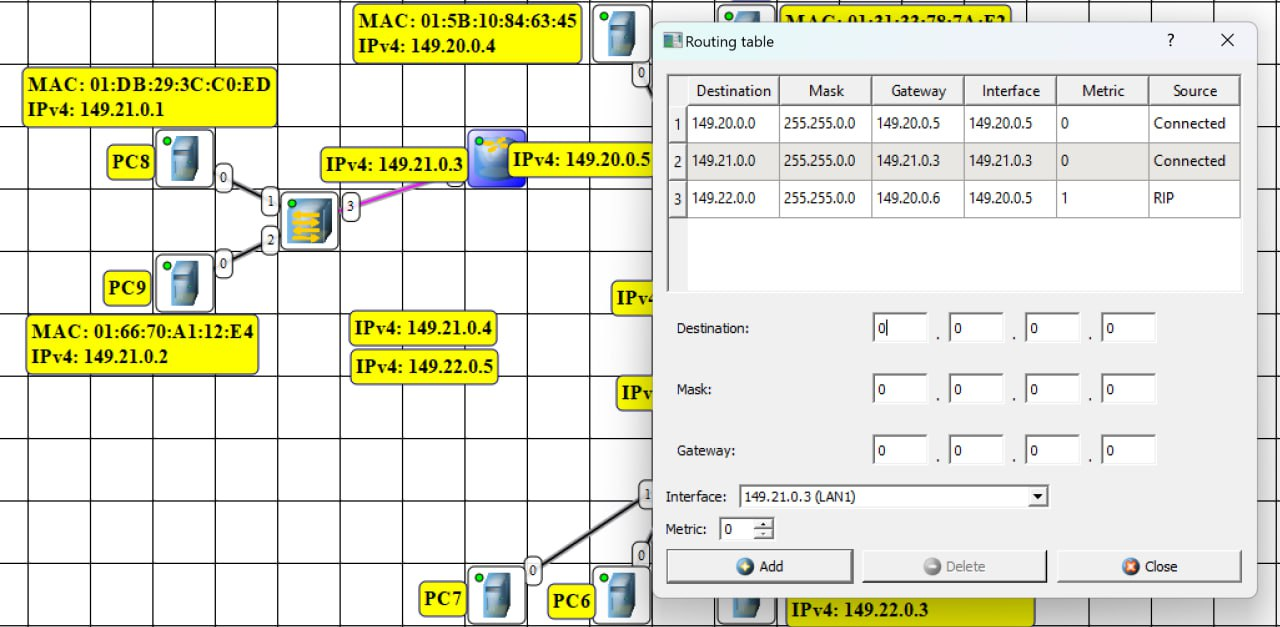
\includegraphics[width=.9\textwidth]{4-0}
\end{center}

\section*{Введение DHCP}
\begin{center}
    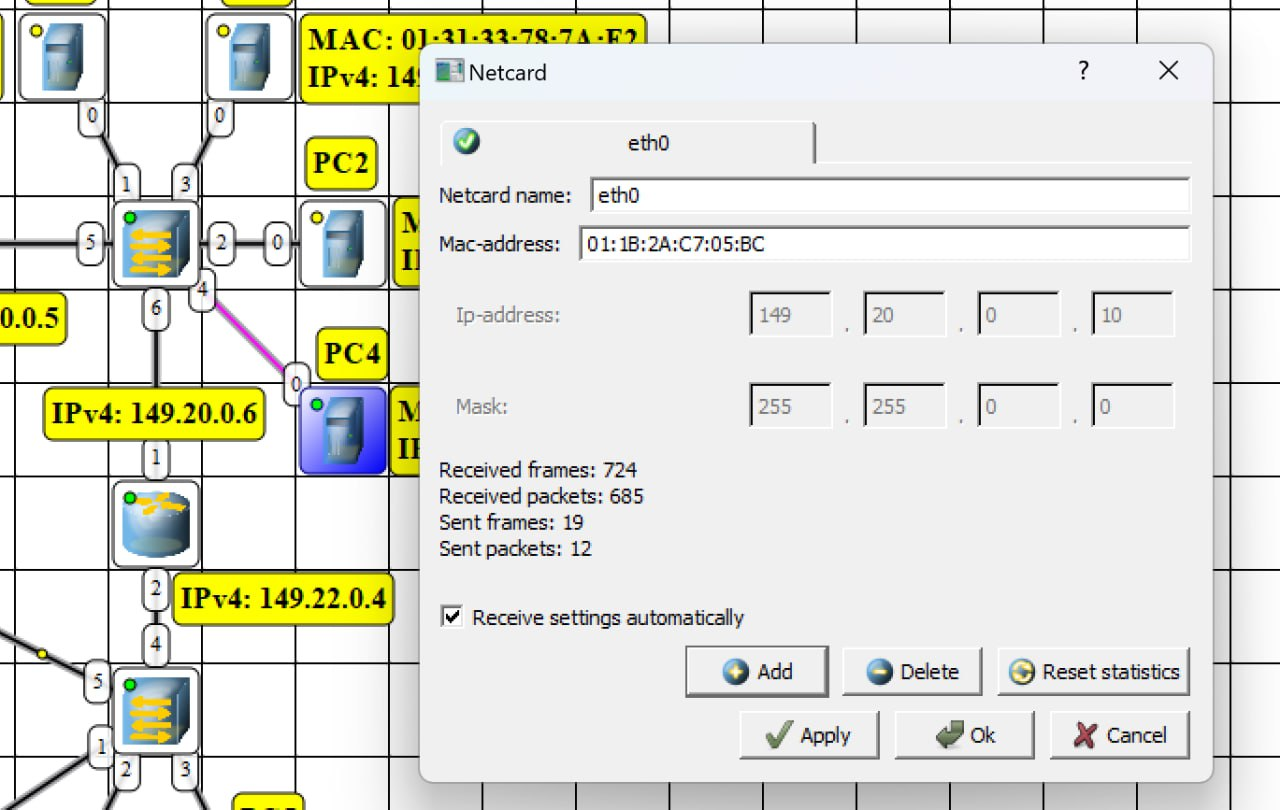
\includegraphics[width=.9\textwidth]{4-1}
\end{center}

\begin{center}
    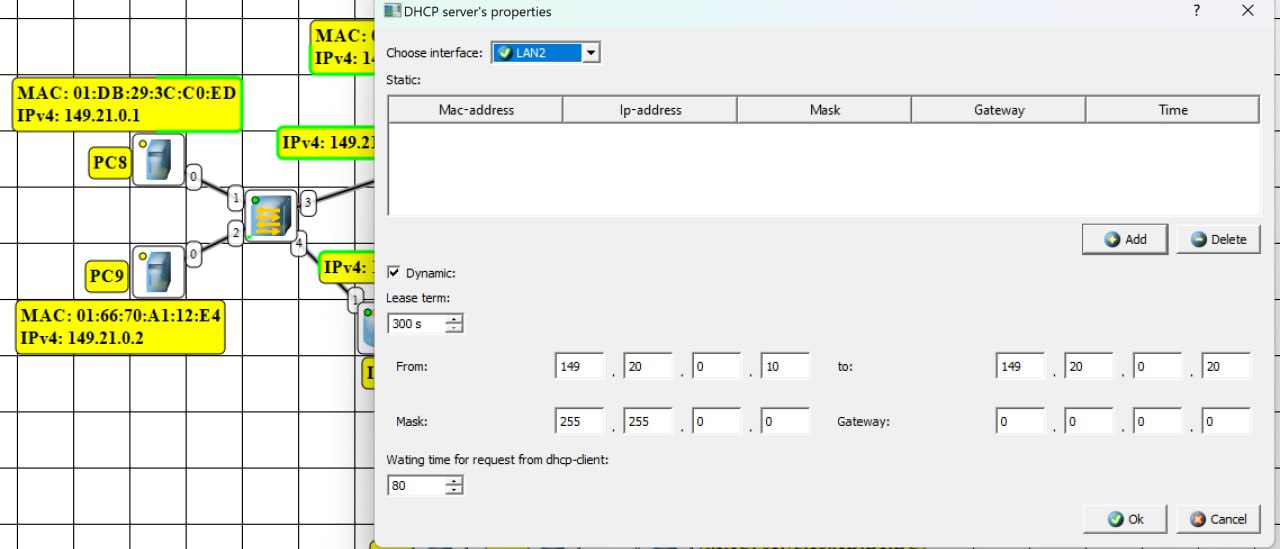
\includegraphics[width=.9\textwidth]{4-2}
\end{center}


\section*{Вывод}
Изучили принципы конфигурирования и процессов функционирования
компьютерных сетей, представляющих собой несколько подсетей, связанных с
помощью маршрутизаторов, процессов автоматического распределения сетевых
адресов, принципов статической маршрутизации и динамической маршрутизации, а также передачи данных на основе протоколов UDP и TCP.

\end{document}

\begin{center}
    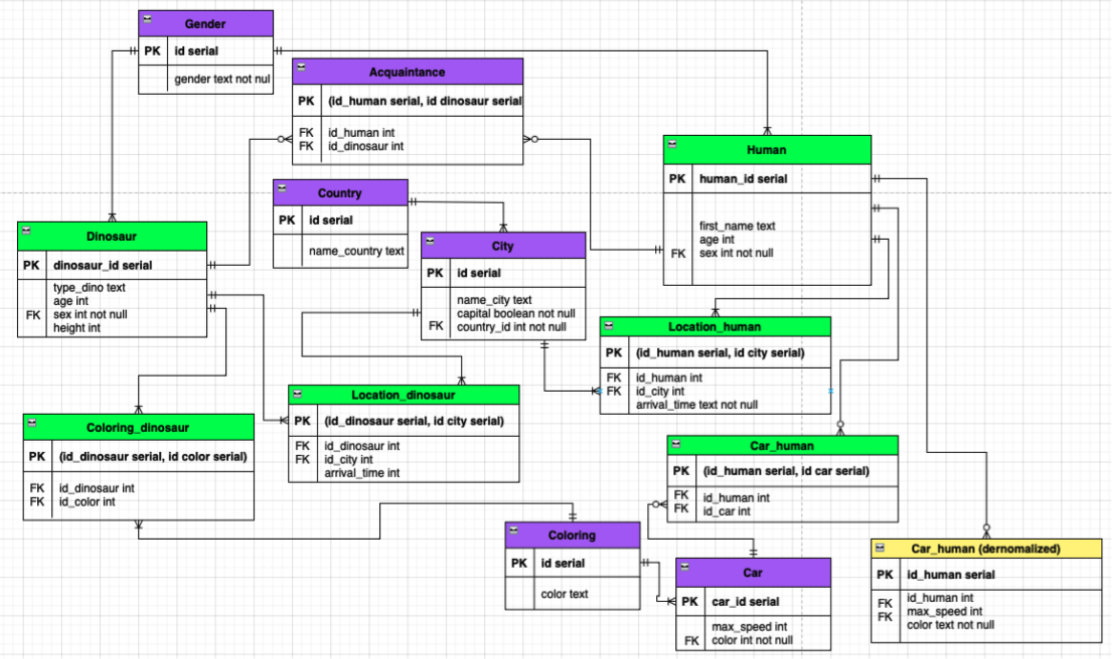
\includegraphics[width=.9\textwidth]{123}
\end{center}